\subsection{Performance along sensitivity curves}

We evaluate the sensitivity curves at $\rho=-0.8,-0.75,\ldots,0.8$, using the same 500 data sets per configuration and identical estimator settings. Curve evaluations remain correlated within each replication; the Monte Carlo sample size is 500, not the number of grid evaluations.

The evaluation uses two complementary targets. If the generating correlation is $r$, the population PNIE/TNIE sensitivity curves in this design are
\begin{equation}
\delta_t^{(r)}(\rho)
=0.4\left\{-0.8+t+r-\frac{\rho}{\sqrt{1-\rho^2}}\sqrt{1-r^2}\right\}.
\label{eq:simulation-sensitivity-truth}
\end{equation}
Curve bias, RMSE and pointwise coverage target \eqref{eq:simulation-sensitivity-truth}; inclusion of the fixed generating effect is recorded separately. The targets coincide at $\rho=r$, distinguishing curve calibration from causal recovery when a different correlation is assumed.

Figure~\ref{fig:simulation-sensitivity-curves} displays PNIE curve estimates and sampling ranges. Figures~S3--S4 and Table~S11 add pointwise coverage, paired RMSE and zero-boundary inference; the project repository retains all effects, correlations, Monte Carlo errors and all-attempted summaries.

\begin{figure}[htbp]
\centering
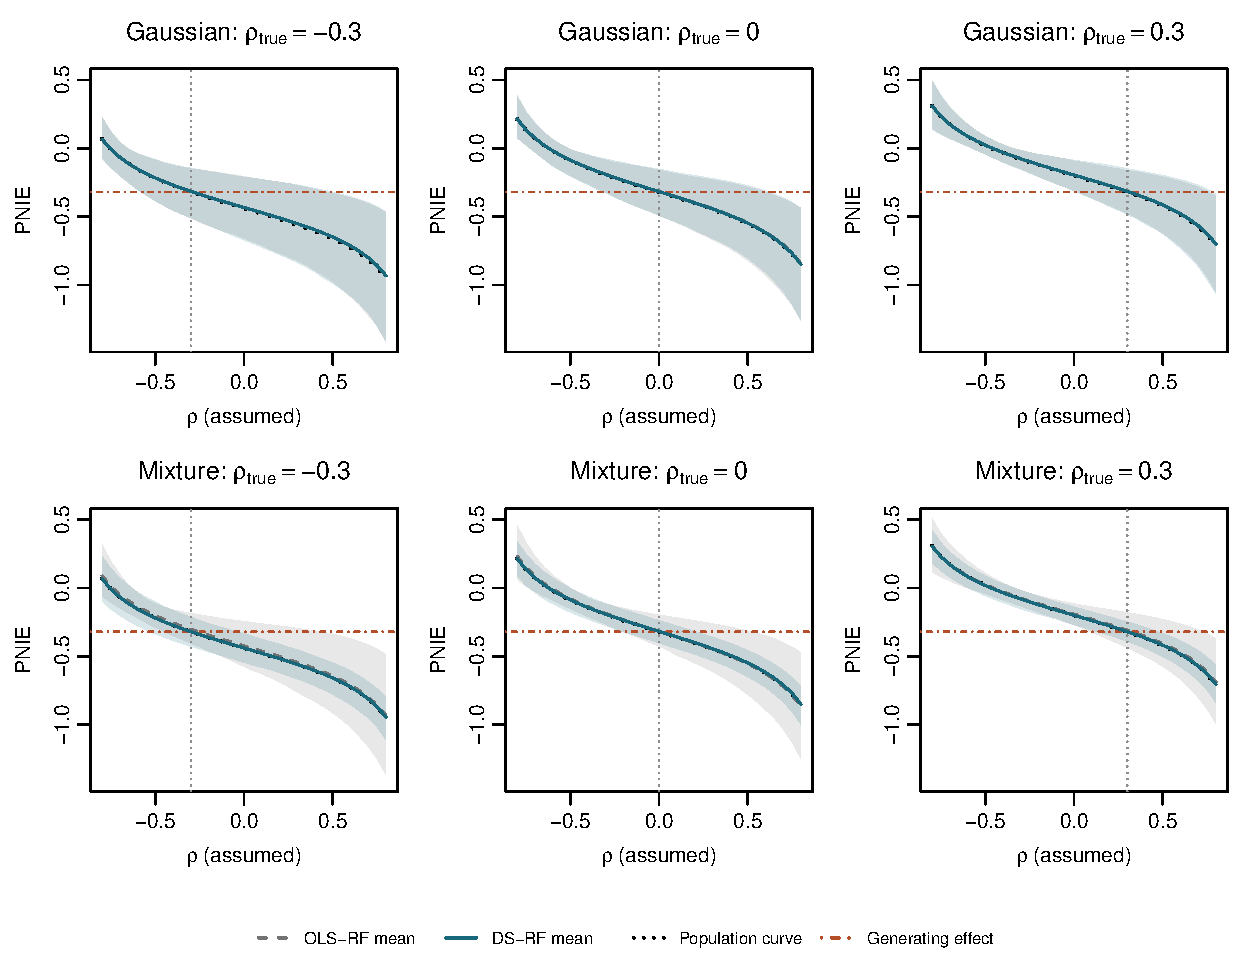
\includegraphics[width=0.98\textwidth]{figures/confounding_simulation_curves.pdf}
\caption{Simulated PNIE sensitivity curves at $n=300$, with 500 attempted replications for each generating correlation and innovation density. Lines show Monte Carlo mean estimates and the population sensitivity curve. Gray and blue shading show central 90\% empirical sampling ranges of the OLS-RF and DS-RF estimates across successful replications, respectively. The horizontal reference is the generating PNIE, $-0.32$, and the vertical reference is the generating correlation. All six configurations are shown.}
\label{fig:simulation-sensitivity-curves}
\end{figure}

Across all three generating correlations and the 33-point grid, paired PNIE RMSE ratios range from 0.985 to 1.054 under Gaussian innovations and from 0.341 to 1.363 under asymmetric-mixture innovations. The asymmetric-mixture results identify regions with substantial precision gains alongside regions with comparable or higher RMSE. Mixture TNIE ratios similarly range from 0.367 to 1.085. This pattern is explained by the nuisance components that dominate the effect gradient: near a zero of $b_t(\rho)$, the derivative of $\delta_t$ with respect to $\beta_2$ is small, whereas regions with a larger derivative can benefit more from precise mediator treatment-effect estimation.

For mixture innovations, DS-RF pointwise curve coverage ranges from 0.924 to 0.966 for PNIE and from 0.904 to 0.964 for TNIE, quantifying the calibration accompanying the precision pattern across the grid. Gaussian coverage likewise varies with the assumed correlation. Zero-boundary RMSE and interval lengths are nearly identical between methods (Table~S11), as predicted by their shared first-order residual-moment representation. Together, the results characterize three complementary features of sensitivity analysis: precision along the assumed-correlation curve, pointwise interval calibration and the point-estimate zero boundary. The separately retained generating-effect inclusion frequencies quantify how recovery of the causal effect depends on the specified confounding value.

\FloatBarrier
